\section{Concrete approaches}\label{approaches}
\subsection{Narratology excursion}
The following two subsections (\ref{fabula} and \ref{discourse}) will showcase two concrete cases of story telling by application of AI planning. Because they approach the subject matter on different levels a distiction is required. It will be necessary to distinguish between \emph{fabula} (or \emph{story}) on the one hand, and \emph{discourse} (or \emph{plot}) on the other hand.\\
Chatman writes in \cite{Chatman1980} (furthermore cited in \cite{Herman10}):
\begin{quote}
''In simple terms, the story is the \emph{what} in a narrative that is depicted, discourse is the \emph{how}.''

(Note: Since \emph{story} and \emph{plot} are more commonly used in everyday language and might lead to confusion or wrong assumptions the remainder of this document will refer to the two concepts as \emph{fabula} and \emph{discourse}.)
\end{quote}
To illustrate the difference with an example: viewers of a movie might be presented with a character A, talking about what a character B has done (assume A's report to be truthful and B's action to be relevant for the movie). On the level of the fabula (the narrative structure), we have B doing something. On the level of the discourse (how this is conveyed to the recipient) we have A talking about it. When watching a movie or reading a book one is presented with a discourse and automatically constructs a fabula in their head.
% - 2 approaches address story/narrative at different levels
% - fabula vs discourse
\subsection{Planning a fabula}\label{fabula}
In \cite{Haslum14} Haslum shows how a specific model of story generation proposed for the IPOCL planner can compiled into a classic planning problem. The model in question is designed to create fabulae and incorporates the notion of character intetions.
\subsubsection{Story world modelling}
% - (desired) story outcome
% - character goals (can change, are influenced by other characters / events)
% - intentional agents (actions percievable as contributing to goals)
% - characters (humans, monsters (genie, dragon))
%     - have given abilities (travel betw. locations, slay monsters, take things from dead, gain control over (genie), fall in love, marry)
%     -> move in world, interact w/ other chars + world/objects
% - intentional actions vs. happenings (e.g. monster frightens human, human falls in love)
% - delegating actions (command, persuade, bribe, ... other char to so sth.)
% - intentional plan
%     -> frame of commitment
% - 
% - 
\subsubsection{Compilations}
% - 
\subsection{Planning a discourse}\label{discourse}
In \cite{Porteous10} Porteous, Cavazza, and Charles
\subsubsection{Story world modelling}
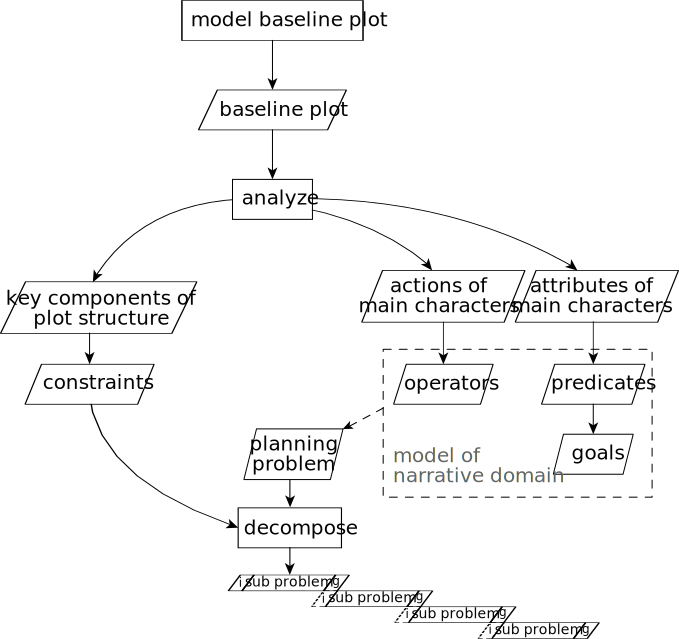
\includegraphics[scale=0.6]{discourse_model}
\subsubsection{Planning}
% - PoV
